Das Scanning Acoustic Microscope (SAM), auch bekannt als akustisches Mikroskop, wurde 1974 an der Stanford University entwickelt und stellte das erste Instrument dar, das in der Lage war, ein akustisches Bild zu erzeugen.\\

Das Grundprinzip der SAM basiert auf einem Wandler (Transducer), der Ultraschallwellen erzeugt. Diese werden mithilfe einer akustischen Linse fokussiert und auf die zu untersuchende Probe gerichtet. Beim Auftreffen auf das Material werden die Wellen absorbiert, reflektiert oder gestreut, abhängig von den Eigenschaften der inneren Strukturen. Die reflektierten Wellen werden von Detektoren – meist oberhalb oder unterhalb der Probe – erfasst und in elektrische Signale umgewandelt.

Diese elektrischen Signale liefern Informationen über materialinterne Eigenschaften wie Schichtdicke, Dichte und Grenzflächenbeschaffenheit. Die verwendeten Frequenzen der Ultraschallwellen sind dabei entscheidend, da sie die Auflösung und Eindringtiefe bestimmen. Je nach Frequenz können innere Strukturen wie Risse, Delaminationen, Lufteinschlüsse oder Hohlräume detektiert werden.

Eine Vielzahl von Materialien, die in der industriellen Fertigung verwendet werden – etwa Silizium, Epoxidharz, Bonding-Materialien und Metallrahmen – übertragen Ultraschallwellen ausreichend gut, um eine bildgebende Analyse zu ermöglichen.\\

Das am häufigsten genutzte Verfahren der SAM ist der Reflexionsmodus (Pulse-Echo-Verfahren). Dabei wird eine Ultraschallwelle in die Probe eingekoppelt. Ein Teil der Welle wird an inneren Grenzflächen reflektiert und gelangt zurück zum Wandler, wo sie erneut in ein elektrisches Signal umgewandelt wird. Die Intensität und Polarität dieser Signale liefern Rückschlüsse auf die inneren Strukturen des untersuchten Materials.
\\



 \newpage
\vspace{0.2cm}
\begin{figure}
    \centering
    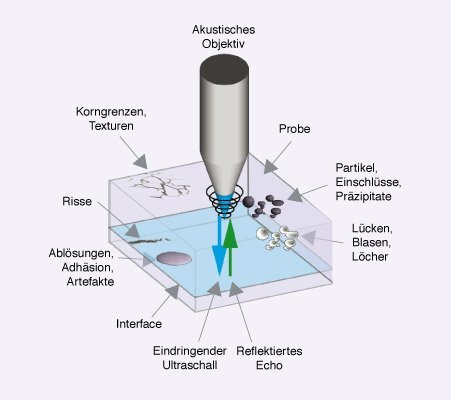
\includegraphics[scale=0.8]{Bilder/samtheorie}
    \caption{Schematische Darstellung des Funktionsprinzips der Scanning Acoustic Microscopy (SAM) im Reflexionsmodus. Die eingestrahlten Ultraschallwellen werden an inneren Strukturen wie Rissen, Grenzflächen, Einschlüsse oder Delaminationen reflektiert und ermöglichen so eine zerstörungsfreie Analyse der Probe.\cite{1}}
    \vspace{0.2cm}
    \label{Abb.1: Schematische Darstellung des Funktionsprinzips der Scanning Acoustic Microscopy (SAM) im Reflexionsmodus. Die eingestrahlten Ultraschallwellen werden an inneren Strukturen wie Rissen, Grenzflächen, Einschlüsse oder Delaminationen reflektiert und ermöglichen so eine zerstörungsfreie Analyse der Probe. }
\end{figure} 
\vspace{0.2cm}
Zur optimalen Übertragung der akustischen Wellen befindet sich die Probe während der Messung in einem Wasserbad. Wasser dient dabei als Kopplungsmedium, da es eine homogene akustische Impedanz aufweist und eine gleichmäßige Grenzfläche zwischen Sonde und Probe bildet.
